\chapter{Neutron Interaction Cross Sections and Sampling Techniques}
\label{ch:neutron_ineractions}
To conduct a Monte Carlo random walk for neutrons the individual reactions that
make up the collision kernel must be discussed. In addition, the methods used
to sample from the differential interaction cross sections must be discussed.
Because of the increased complexity of reactions between a neutron and an a
atomic nucleus compared to photon-atomic reactions, closed form differential
interaction cross sections are quite rare. The models and procedures that are
outlined in the ENDF manual will therefore be relied upon heavily. In this
chapter all secondary particles other than neutrons will be neglected from the
cross sections and sampling procedures. 

\section{Elastic and Inelastic Level Scatering}
Elastic and inelastic level scattering are the two simplest scattering reactions
between a neutron and an atomic nucleus. In elastic scattering the internal 
state of the atomic nucleus is left unchanged. In inelastic level scattering 
the atomic nucleus is excited to a particular state, which has an energy that 
will be denoted as Q above the ground state. Elastic scattering can therefore 
be regarded as a special case of inelastic scattering with Q set equal to zero.
Because of the complicated nature of the interaction between a neutron and the
atomic nucleus it is difficult to develop an equation for the differential
elastic or inelastic level scattering cross section for all incoming neutron 
energies. The solution to this problem is to develop tabulated angular 
distributions for a range of incoming neutron energies, which can be found in 
the ENDF/B-VII.1 library \citep{chadwick_endf/b-vii.1_2011}. 

According to the ENDF/B-VII.1 manual, the angular distrubitions for elastic and 
inelastic level scattering are expressed as normalized probability 
distributions.
\begin{equation}
  p(\mu,E^{'}) = \frac{2\pi}{\sigma(E^{'})}\sigma(\mu,E^{'})
\end{equation}
\begin{equation}
  \int_{-1}^1p(\mu,E^{'})d\mu=1
\end{equation}
The angular distribition will be given in either a tabular form or as a 
Legendre polynomial series, which is shown below.
\begin{equation}
  p(\mu,E^{'}) = \sum_{l=0}^N\frac{2l+1}{2}a_l(E^{'})P_l(\mu)
\end{equation}
In addition, the outgoing angle cosine can be given in either the lab frame or
the center-of-mass (CM) frame. However, for two-body reactions like elastic and 
inelastic level scattering the scattering angle cosine will usually be given in 
the CM frame \citep{chadwick_endf/b-vii.1_2011}. 

Sampling an outgoing angle from the PDF given in the ENDF library can be done 
in many ways \citep{lux_monte_1991}. In older Monte Carlo codes, including older
versions of MCNP, the most common sampling technique was that proposed by 
Carter and Cashwell in which n equally probable intervals of the CDF are 
tabulated \citep{l._l._particle-transport_1975}. To select an outgoing angle 
cosine, one randomly selects an interval of the CDF and then selects the 
scattering angle cosine from a uniform PDF between the lower and upper 
boundaries of the selected interval \citep{lux_monte_1991}. This method is very 
computationally efficient but can become inaccurate when the PDF is given as a 
Legendre polynomial with many higher order terms 
\citep{x-5_monte_carlo_team_mcnp_2003}. The next best option is to use a 2-D 
tabular selection method \citep{x-5_monte_carlo_team_mcnp_2003}. This is very
similar to the tabular selection method which was discussed in the previous 
chapter. At each of the selected incoming neutron energies the CDF corresponding
to the PDF given in the ENDF library must first be calculated. To sample an 
outgoing angle cosine corresponding to a particular incoming neutron energy one
must determine which energy bin the neutron's energy falls in, which can be 
accomplished with a binary search. Then one samples a random number and 
for the distribution corresponding to both energy bin boundaries, determines 
the outgoing angle cosine corresponding to that CDF value. The outgoing angle
cosine corresponding to the incoming energy must then be found using
interpolation between the two values. A set of appropriate interpolation schemes
for 2-D tables are given in the ENDF/B-VII.1 manual 
\citep{chadwick_endf/b-vii.1_2011}. 

Once the CM scattering angle cosine is sampled, it must be converted to the 
lab scattering angle cosine. This equation, which is shown below, can be derived
using conservation of energy and momentum in both reference frames (see 
Appendix \ref{ch:appendix_C}).
\begin{equation}
  \mu_{l} = \frac{A\sqrt{1-\left(\frac{A+1}{A}\right)\frac{Q}{E^{'}}}\mu_{cm} + 1}
  {\sqrt{A^2\left[1-\left(\frac{A+1}{A}\right)\frac{Q}{E^{'}}\right] + 
      2A\mu_{cm}\sqrt{1-\left(\frac{A+1}{A}\right)\frac{Q}{E^{'}}} + 1}}
  \label{eq:lab_scatterin_angle_cosine}
\end{equation}
\begin{equation*}
  A = \frac{m_A}{m_n}
\end{equation*}

Because of the one-to-one correspondence between the outgoing energy and
outgoing direction in the two-body reactions, once the outgoing angle cosine
has been sampled the outgoing energy of the neutron can be determined. The
equations that described this one-to-one correspondence can be found using
conservation of energy and momentum and the assumption that the atomic nucleus
upon which the neutron scatters is at rest. The outgoing energy from an 
inelastic level scattering interaction (in the lab frame) as a function of the 
initial energy and the scattering angle in the center of mass system is the 
following (see Appendix \ref{ch:appendix_C}).
\begin{equation}
  E = E^{'} \left(\frac{A^2\left[1-\left(\frac{A+1}{A}\right)\frac{Q}{E^{'}}
      \right]+ 2A\mu_{cm}\sqrt{1 - \left(\frac{A+1}{A}\right)\frac{Q}{E^{'}}}
     + 1}{\left(A+1\right)^2}\right) 
  \label{eq:neutron_outgoing_energy}
\end{equation}
The outgoing energy is limited to the following range.
\begin{equation}
  \left(\frac{A\sqrt{1-\left(\frac{A+1}{A}\right)\frac{Q}{E}}-1}{A+1}\right)^2
  E^{'} \leq E \leq 
  \left(\frac{A\sqrt{1-\left(\frac{A+1}{A}\right)\frac{Q}{E}}+1}{A+1}\right)^2
    E^{'}
\end{equation}
The lower limit occurs when $\mu_{cm} = -1$ and the upper limit occurs when
$\mu_{cm} = 1$.

\section{Absorption Reactions}
A neutron absorption reaction is any reaction in which an incident neutron is
absorbed and another particle, whether a gamma ray, proton, alpha particle or
some other atomic nucleus, is emitted. When neutrons are the only particle of
interest, these reactions will all be combined into a single absorption
reaction. However, in coupled particle transport calculations, these reactions
along with the neutron collision density will function as the source term for
the other particles of interest. Some of these reactions will be discussed 
further in the following chapter when coupled neutron-photon transport will
be discussed. 

\section{Other Non-fission Reactions}
There are many other reactions which can also be important but are more
complicated than the previous reactions that have been discussed. A few 
examples are the inelastic scattering to a continuum of energy levels, the 
(n,2n) reaction and the (n,3n) reaction. For a complete list of possible
non-fission reactions, refer to the ENDF/B-VII.1 manual. In these reactions 
there is assumed to be no correlation between the outgoing energy and direction 
according to the ENDF/B-VII.1 manual \citep{chadwick_endf/b-vii.1_2011}. This 
simplification of the reaction model means that conservation of energy and 
momentum will likely be violated during a given reaction modeled during the
Monte Carlo random walk process. However the average of many individual 
reactions will still give the desired behavior. The neutron transfer 
probability for any of these reactions can be represented as follows.
\begin{align}
  f(E^{'} \to E,\hat{\Omega}^{'} \to \hat{\Omega}) & = p(E^{'} \to E)
  p(\hat{\Omega}^{'} \to \hat{\Omega} | E^{'}) \nonumber \\
  & = p(E^{'} \to E)p(\hat{\Omega}^{'}\cdot\hat{\Omega} | E^{'}) \nonumber \\
  & = p(E^{'} \to E)p(\mu,E^{'})
\end{align}

As with elastic and inelastic level scattering the angular distributions are
expressed as normalized PDFs 
\citep{chadwick_endf/b-vii.1_2011}. 
\begin{equation*}
  p(\mu,E^{'}) = \frac{2\pi}{\sigma(E^{'})}\sigma(\mu,E^{'})
\end{equation*}
\begin{equation*}
  \int_{-1}^1p(\mu,E^{'})d\mu = 1
\end{equation*}
In addition the angular distrubition will be given in either a tabular form or
as a Legendre polynomial series. Usually, the outgoing angle cosine for these
reactions will be given in the lab frame \citep{chadwick_endf/b-vii.1_2011}. To
sample an outgoing angle cosine, the same tabular procedure that was outlined 
in the previous section should be used. 

The energy distributions are also expressed as normalized PDFs 
\citep{chadwick_endf/b-vii.1_2011}. The variable c is the number of neutrons
emitted from the reaction.
\begin{equation}
  p(E^{'} \to E) = \frac{1}{c\sigma(E^{'})}\frac{d\sigma(E^{'} \to E)}{dE}
\end{equation}
\begin{equation}
  \int_0^{E_{max}}p(E^{'} \to E)dE = 1
\end{equation}
The energy distributions are given in either a tabular form or as an analytical
formulation. The possible analytical formulations are the general evaporative
spectrum or the evaporation spectrum \citep{chadwick_endf/b-vii.1_2011}. The 
general evaporative spectrum has the following form.
\begin{equation}
  p(E^{'} \to E) = g(E/\theta(E^{'}))
\end{equation}
The function $\theta(E^{'})$ is tabulated as a function of incident neutron 
energy and the function $g(x)$ is tabulated as a function of 
$x = E/\theta(E^{'})$. To sample from this function a CDF corresponding to 
the pdf g(x) must be created. One then samples a random number and finds the
value of x that corresponds to the random number in the CDF that was 
calculated. Finally, the outgoing energy is calculated as follows.
\begin{equation}
  E = x\theta(E^{'})
\end{equation}

The evaporation spectrum, which is used for most non-fission reactions, has the following form \citep{chadwick_endf/b-vii.1_2011}.
\begin{equation}
  p(E^{'} \to E) = \frac{E}{I}exp\left[\frac{-E}{\theta(E^{'})}\right]
\end{equation}
\begin{equation}
  I = \theta^2(E^{'})\left[1 - exp\left[\frac{-(E^{'}-U)}{\theta(E^{'})}\right]
    \left(1+\frac{E^{'}-U}{\theta(E^{'})}\right)\right]
\end{equation}
The function $\theta(E^{'})$ is again tabulated as a function of incident
neutron energy and the variable U is introduced to define the proper upper 
limit for the final particle energy. Sampling from this distribution is also
quite simple. However, the derivation of the sampling procedure is slightly
complicated. Consider another PDF that has the same shape as the 
evaporation spectrum but extends to infinity (instead of $E^{'}-U$). 
\begin{equation}
  f(E^{'} \to E) = \frac{E}{\theta^2(E^{'})}exp\left[\frac{-E}{\theta(E^{'})}
    \right]
\end{equation}
Also assume that the energy E is the sum of two values $E_1$ and $E_2$, which
are independent of each other. If the PDF corresponding to $E_1$ is
\begin{equation}
  f_1(E^{'} \to E_1) = \frac{1}{\theta(E^{'})}exp\left[\frac{-E_1}{\theta(E^{'})}
    \right]
\end{equation}
and the PDF corresponding to $E_2$ is 
\begin{equation}
  f_2(E^{'} \to E_2) = \frac{1}{\theta(E^{'})}exp\left[\frac{-E_2}{\theta(E^{'})}
    \right]
\end{equation}
then the PDF for E is the following \citep{kahn_applications_1956}.
\begin{align}
  f(E^{'} \to E) & = \int_0^{E}f_1(E^{'} \to E-E_2)f_2(E^{'} \to E_2) dE_2 \\
  & = \frac{1}{\theta^2(E^{'})}\int_0^{E} exp\left[\frac{-(E-E_2)}{\theta(E^{'})}
    \right] exp\left[\frac{-E_2}{\theta(E^{'})}\right] dE_2 \nonumber \\
  & = \frac{1}{\theta^2(E^{'})} exp\left[\frac{-E}{\theta(E^{'})}\right]
  \int_0^{E} dE_2 \nonumber \\
  & = \frac{E}{\theta^2(E^{'})}exp\left[\frac{-E}{\theta(E^{'})}\right] \nonumber
\end{align}
Both $E_1$ and $E_2$ can be sampled from their respective PDFs using the
inverse CDF method. 
\begin{align}
  E_1 & = -\theta(E^{'})\ln{\varepsilon_1} \\
  E_2 & = -\theta(E^{'})\ln{\varepsilon_2} 
\end{align}
Since E is the sum of these two values, the equation for sampling E directly
is the following \citep{x-5_monte_carlo_team_mcnp_2003}.
\begin{align}
  E & = E_1 + E_2 \nonumber \\
  & = -\theta(E^{'})\ln{(\varepsilon_1\varepsilon_2)}
\end{align}
Finaly, since E was sampled from a distrubition that wasn't truncated properly,
the value of E must be rejected if it is greater than $E^{'}-U$ to account for
the improper truncation.

\section{Neutron Induced Fission}
Fission reaction must also be taken into account since for the random walk
procedure that has been described, fission can occur as long as the system is
subcritical. In fission reactions there is also assumed to be no correlation
between outgoing energy and direction according to the ENDF/B-VII.1 manual
\citep{chadwick_endf/b-vii.1_2011}. The neutron transfer probability for 
fission reactions will therefore have the same form as for the non-fission
reactions from the previous section. 

The energy distributions are again expressed as normalized PDFs
\citep{chadwick_endf/b-vii.1_2011}. The variable $\nu(E^{'})$ is the average 
number of either prompt or delayed neutrons emitted by the fission reaction, 
depending on which distribution is of interest. 
\begin{equation}
  p(E^{'} \to E) = \frac{1}{\nu(E^{'})\sigma_f(E^{'})}
  \frac{d\sigma_f(E^{'} \to E)}{dE}
\end{equation}
\begin{equation}
  \int_0^{E_{max}}p(E^{'} \to E)dE = 1
\end{equation}
The energy distributions are given in either a tabular form or as an analytical
formulation. The possible analytical formulations are the evaporation spectrum, 
which was discussed in the previous section, the simple Maxwellian fission 
spectrum and the energy-dependent Watt spectrum 
\citep{chadwick_endf/b-vii.1_2011}. The simple Maxwellian fission spectrum has 
the following form.
\begin{equation}
  p(E^{'} \to E) = \frac{\sqrt{E}}{I}exp\left[\frac{-E}{\theta(E^{'})}\right]
\end{equation}
\begin{equation}
  I = \theta^{3/2}(E^{'})\left[\frac{\sqrt{\pi}}{2}
    erf\left(\sqrt{\frac{(E^{'}-U)}{\theta(E^{'})}}\right) -
    \sqrt{\frac{(E^{'}-U)}{\theta(E^{'})}}
    exp\left[\frac{-(E^{'}-U)}{\theta(E^{'})}
      \right]\right]
\end{equation}
The function $\theta(E^{'})$ is tabulated as a function of incident neutron
energy and the variable U is introduced to define the proper upper limit for 
the final particle energy. In the case of fission reactions, U is usually a
large negative number since the outgoing neutrons can have an energy much 
higher than the incoming neutron \citep{chadwick_endf/b-vii.1_2011}. Several
methods are commonly used to sample from this distribution. All methods assume
that the outgoing enegy can take on any value between zero and infinity, which
results in a slightly different normalization of the distribution. The
Maxwellian distribution falls off quickly enough that this difference is
neglibible. 

The first method for sampling from the Maxwellian is a direct sampling method, 
which is shown in the following equation \citep{mohamed_efficient_2011}.
\begin{equation}
  E = -\theta(E^{'})\left[cos^2\left(\frac{2}{\pi}\varepsilon_1\right)
    \ln{\varepsilon_2} + \ln{\varepsilon_3}\right]
\end{equation}
For a derivation of this method, refer to appendix \ref{ch:Appendix_C}. The
second method is a rejection sampling procedure. It is referred to by
some authors as Johnk's algorithm\footnote{This method is used in MCNP 
\citep{x-5_monte_carlo_team_mcnp_2003}.} and is shown in figure 
\ref{fig:Johnks_algorithm} \citep{mohamed_efficient_2011, c._j._everett_third_1983}. 
\begin{figure}[t!]
  \begin{center}
    \def\svgwidth{170bp}
    \input{chapters/neutron_interactions/Johnks_algorithm.pdf_tex}
  \end{center}
  \caption{\textbf{Johnk's Algorithm}.
    \textit{This sampling procedure is used to sample a value from the 
      Maxwellian distribution. The efficiency of this procedure is about
      0.78 and is independent of the incoming neutron energy 
      \citep{mohamed_efficient_2011}.}}
  \label{fig:Johnks_algorithm}
\end{figure}
The derivation of this method can also be found in appendix \ref{ch:Appendix_C}.
The final sampling method is also a rejection sampling procedure, which is shown
in figure \ref{fig:Mohameds_rejection_sampling_procedure}. 
\begin{figure}[t!]
  \begin{center}
    \def\svgwidth{120bp}
    \input{chapters/neutron_interactions/Mohameds_rejection_sampling_proc.pdf_tex}
  \end{center}
  \caption{\textbf{Mohamed's Rejection Sampling Procedure}.
    \textit{This sampling procedure is used to sample a value from the
      Maxwellian distribution. The efficiency of this procedure is about
      0.73 and is independent of the incoming neutron energy
      \citep{mohamed_efficient_2011}.}}
  \label{fig:Mohameds_rejection_sampling_procedure}
\end{figure}
Mohamed has shown that this method is the fastest of the three for generating 
random samples from a Maxwellian distribution despite having an efficiency of 
only 0.73 \citep{mohamed_efficient_2011}. The derivation of this method can 
also be found in appendix \ref{ch:Appendix_C}.

The energy energy-dependent Watt spectrum has the following form.
\begin{equation}
  p(E^{'} \to E) = I^{-1}exp\left[\frac{-E}{a(E^{'})}\right]
  sinh\left(\sqrt{b(E^{'})E}
  \right)
\end{equation}
\begin{align}
  I & = \frac{1}{2}\sqrt{\frac{\pi a^3b}{4}}exp\left(\frac{ab}{4}\right)\left[
    erf\left(\sqrt{\frac{E^{'}-U}{a}} - \sqrt{\frac{ab}{4}}\right) +
    erf\left(\sqrt{\frac{E^{'}-U}{a}} + \sqrt{\frac{ab}{4}}\right)\right] 
  \nonumber \\
  & \qquad - a \exp{\left[-\left(\frac{E^{'}-U}{a}\right)\right]}
  sinh\sqrt{b(E^{'}-U)}
\end{align}
The functions $a(E^{'})$ and $b(E^{'})$ are tabulated as a function of incident 
neutron energy and the variable U is introduced to again define the proper 
upper limit for the final particle energy. Two methods are commonly used to
sample from this distribution. Both methods assume that the outgoing energy
can take on any value between zero and infinity, which results in a slightly
different normalization of the distribution. However, the distribution falls
off quickly enough thta this difference is negligible.

The first method is rejection sampling procedure referred to as Kalos's 
algorithm \citep{mohamed_efficient_2011}. This method is shown in figure
\ref{fig:Kalos_algorithm}. 
\begin{figure}[t!]
  \begin{center}
    \def\svgwidth{190bp}
    \input{chapters/neutron_interactions/Kalos_algorithm.pdf_tex}
  \end{center}
  \caption{\textbf{Kalos's Algorithm}.
    \textit{This sampling procedure is used to sample a value from the
      Watt fission spectrum. The efficiency of this procedure is about
      0.67 and is independent of the incoming neutron energy
      \citep{mohamed_efficient_2011}.}}
  \label{fig:Kalos_algorithm}
\end{figure}
The efficiency of this method is about 0.67. The 
second method is a direct sampling method, which is shown in the following
equation \citep{mohamed_efficient_2011}. The variable $y$ is a random number
from a Maxwellian distribution with $\theta(E^{'})$ replaced with $a(E^{'})$.
To generate this random number, any of the methods for sampling from a 
Maxwellian distribution can be used. 
\begin{equation}
  E = y + \frac{a^2b}{4} + (2\varepsilon_1-1)\sqrt{a^2by}
\end{equation}
When combined with Mohamed's rejection sampling procedure, the direct sampling
method is the fastest at generating random samples from the Watt spectrum
\citep{mohamed_efficient_2011}.

\section{Thermal Scattering}
In all previous sections it was assumed that the energy of the neutron was
much greater than the thermal energy of the atoms upon which the neutron
interacts. When the neutron energy drops below about one eV, this assumption
is no longer valid. To account for the thermal motion of atoms upon which
the neutron scatters, several models have been developed. 

The most detailed model is the $S(\alpha,\beta)$ model, which can treat thermal 
neutron scattering by both molecules and crystalline solids 
\citep{bell_nuclear_1979, chadwick_endf/b-vii.1_2011}. The $S(\alpha,\beta)$
data required for this model is only available for a few materials in the 
ENDF ENDF/B-VII.1 library \citep{chadwick_endf/b-vii.1_2011}. 

When $S(\alpha,\beta)$ data is not available for a particular material another 
model that can lead to an accurate representation of thermal scattering is
the free gas model. In this model, the atoms upon which the neutrons interact
are assumed to be unbound with speeds characterized by a Maxwell-Boltzmann
distribution \citep{bell_nuclear_1979}. This model is applicable to any
mixture of materials as long as all scattering cross sections are independent
of the relative speed of the neutron and scattering nucleus and all 
effective absoption cross sections are known \citep{bell_nuclear_1979}. 

The final model, which is the simplest and least accurate, is the one-velocity
thermal energy group model. As its name implies, thermal neutrons are treated
as if they all have the same energy with cross sections averaged over this
thermal energy group used. Once a neutron scatters into the thermal group, its
energy never changes due to scattering collisions and therefore, it never leaves
the thermal group. Will many inaccuracies can arrise from this model, the
largest is most likely from the generation of the average cross sections, which
requires an assumption of the thermal neutron spectrum. Despite these
limitations, this model will be employed initially because of the ease with
which an equivalent adjoint model can be created. The development of 
equivalent adjoint models for the other two models will be one of the primary
focuses of the thesis.

The energy transfer probability for elastic scattering for the one-velocity 
thermal energy model is the following \citep{hoogenboom_adjoint_1977}.
\begin{equation}
  p(E^{'} \to E) = \delta(E - E^{'})
\end{equation}
As soon as the neutron scatters to an energy below $E_c$, which is the energy
cutoff for the thermal energy group, its energy will never change. Furthermore,
the cross sections used will be the thermal group averaged cross sections,
which are independent of the actual energy of the thermal neutron. 

\section{Adjoint Elastic and Inelastic Level Scattering}
To model adjoint elastic and inelastic level scattering, the adjoint energy
transfer probabilities and adjoint cross sections must be determined. For
elastic and inelastic level scattering, the double differential transfer
probability is represented by the following function 
\citep{hoogenboom_adjoint_1977}.
\begin{equation}
  p(E^{'} \to E, \mu_{cm}) = p(\mu_{cm},E^{'})\delta\left(E - 
  E^{'} \left(\frac{A^2\left[1-\left(\frac{A+1}{A}\right)\frac{Q}{E^{'}}
      \right]+ 2A\mu_{cm}\sqrt{1 - \left(\frac{A+1}{A}\right)\frac{Q}{E^{'}}}
     + 1}{\left(A+1\right)^2}\right)\right)
\end{equation}
The delta function in the above equation comes about from the one-to-one 
correspondence between the outgoing energy and outgoing direction. The energy
transfer probability can now be deterimed by the following integral.
\begin{equation}
  p(E^{'} \to E) = \int_{-1}^1 p(E^{'} \to E, \mu_{cm}) d\mu_{cm}
\end{equation}
Given that the delta function in the equation for the double differential
transfer probability is in terms of the outgoing energy, the above integral
will be more easily evaluated when the integration is over the outgoing energy.
Based on equation \ref{eq:neutron_outgoing_energy},
\begin{equation}
  d\mu_{cm} = \frac{(A+1)^2}{2AE^{'}\sqrt{1-\left(\frac{A+1}{A}\right)
      \frac{Q}{E^{'}}}} dE.
\end{equation}
Using the change of variables, the energy transfer probability is the following.
\begin{align}
  p(E^{'} \to E) & = \int_{-1}^1 p(E^{'} \to E, \mu_{cm}) 
  \frac{(A+1)^2}{2AE^{'}\sqrt{1-\left(\frac{A+1}{A}\right)\frac{Q}{E^{'}}}} dE
  \nonumber \\
  & = p(E^{'}, \mu_{cm}(E^{'},E)) 
  \frac{(A+1)^2}{2AE^{'}\sqrt{1-\left(\frac{A+1}{A}\right)\frac{Q}{E^{'}}}}
\end{align}

The adjoint elastic and inelastic level scattering cross sections can now be
determined using equation \ref{eq:adjoint_cross_section}.
\begin{equation}
  \sigma_{e/i}^{\dagger}(E^{'}) = \int_{E_{min}}^{E_{max}} \sigma_{e/i}(E)p(E \to E^{'})
    dE
\end{equation}
The last missing piece of information that is needed before the adjoint cross
section can be evaluated is the limits of integrations. These limits can be
determined by determining an equation for the incoming energy as a function of
the outgoing energy (in the forward case). Unfortunately, one cannot simply
solve equation \ref{eq:neutron_outgoing_energy} for $E^{'}$. As figure
\ref{fig:in_out_energies_cm} shows, when the outgoing energy is less than
$\frac{Q}{A(A+1)}$ and the CM scattering angle cosine is less than zero, there 
is not a one-to-one correspondance between incoming energy and the CM 
scattering angle cosine for fixed outgoing energy. If the outgoing energy is 
given as a function of incoming energy and the lab scattering angle instead, as 
shown in figure \ref{fig:in_out_energies_cm}, there is a one-to-one 
correspondance between incoming energy and the lab scattering angle cosine for 
fixed outgoing energy.
\begin{figure}[t!]
  \begin{center}
    % GNUPLOT: LaTeX picture with Postscript
\begingroup
  \makeatletter
  \providecommand\color[2][]{%
    \GenericError{(gnuplot) \space\space\space\@spaces}{%
      Package color not loaded in conjunction with
      terminal option `colourtext'%
    }{See the gnuplot documentation for explanation.%
    }{Either use 'blacktext' in gnuplot or load the package
      color.sty in LaTeX.}%
    \renewcommand\color[2][]{}%
  }%
  \providecommand\includegraphics[2][]{%
    \GenericError{(gnuplot) \space\space\space\@spaces}{%
      Package graphicx or graphics not loaded%
    }{See the gnuplot documentation for explanation.%
    }{The gnuplot epslatex terminal needs graphicx.sty or graphics.sty.}%
    \renewcommand\includegraphics[2][]{}%
  }%
  \providecommand\rotatebox[2]{#2}%
  \@ifundefined{ifGPcolor}{%
    \newif\ifGPcolor
    \GPcolorfalse
  }{}%
  \@ifundefined{ifGPblacktext}{%
    \newif\ifGPblacktext
    \GPblacktexttrue
  }{}%
  % define a \g@addto@macro without @ in the name:
  \let\gplgaddtomacro\g@addto@macro
  % define empty templates for all commands taking text:
  \gdef\gplbacktext{}%
  \gdef\gplfronttext{}%
  \makeatother
  \ifGPblacktext
    % no textcolor at all
    \def\colorrgb#1{}%
    \def\colorgray#1{}%
  \else
    % gray or color?
    \ifGPcolor
      \def\colorrgb#1{\color[rgb]{#1}}%
      \def\colorgray#1{\color[gray]{#1}}%
      \expandafter\def\csname LTw\endcsname{\color{white}}%
      \expandafter\def\csname LTb\endcsname{\color{black}}%
      \expandafter\def\csname LTa\endcsname{\color{black}}%
      \expandafter\def\csname LT0\endcsname{\color[rgb]{1,0,0}}%
      \expandafter\def\csname LT1\endcsname{\color[rgb]{0,1,0}}%
      \expandafter\def\csname LT2\endcsname{\color[rgb]{0,0,1}}%
      \expandafter\def\csname LT3\endcsname{\color[rgb]{1,0,1}}%
      \expandafter\def\csname LT4\endcsname{\color[rgb]{0,1,1}}%
      \expandafter\def\csname LT5\endcsname{\color[rgb]{1,1,0}}%
      \expandafter\def\csname LT6\endcsname{\color[rgb]{0,0,0}}%
      \expandafter\def\csname LT7\endcsname{\color[rgb]{1,0.3,0}}%
      \expandafter\def\csname LT8\endcsname{\color[rgb]{0.5,0.5,0.5}}%
    \else
      % gray
      \def\colorrgb#1{\color{black}}%
      \def\colorgray#1{\color[gray]{#1}}%
      \expandafter\def\csname LTw\endcsname{\color{white}}%
      \expandafter\def\csname LTb\endcsname{\color{black}}%
      \expandafter\def\csname LTa\endcsname{\color{black}}%
      \expandafter\def\csname LT0\endcsname{\color{black}}%
      \expandafter\def\csname LT1\endcsname{\color{black}}%
      \expandafter\def\csname LT2\endcsname{\color{black}}%
      \expandafter\def\csname LT3\endcsname{\color{black}}%
      \expandafter\def\csname LT4\endcsname{\color{black}}%
      \expandafter\def\csname LT5\endcsname{\color{black}}%
      \expandafter\def\csname LT6\endcsname{\color{black}}%
      \expandafter\def\csname LT7\endcsname{\color{black}}%
      \expandafter\def\csname LT8\endcsname{\color{black}}%
    \fi
  \fi
  \setlength{\unitlength}{0.0500bp}%
  \begin{picture}(7200.00,5040.00)%
    \gplgaddtomacro\gplbacktext{%
      \csname LTb\endcsname%
      \put(792,1383){\makebox(0,0)[r]{\strut{}$\frac{Q}{A(A+1)}$}}%
      \csname LTb\endcsname%
      \put(792,484){\makebox(0,0){\strut{}$\frac{A+1}{A}Q$}}%
      \csname LTb\endcsname%
      \put(2796,484){\makebox(0,0){\strut{}$\frac{A}{A-1}Q$}}%
      \put(576,2739){\rotatebox{-270}{\makebox(0,0){\strut{}Outgoing Energy}}}%
      \put(3797,154){\makebox(0,0){\strut{}Incoming Energy}}%
      \put(5601,1030){\makebox(0,0)[l]{\strut{}$\mu_{cm} = -1$}}%
      \put(5601,2332){\makebox(0,0)[l]{\strut{}$\mu_{cm} = -\frac{1}{2}$}}%
      \put(5000,3676){\makebox(0,0)[l]{\strut{}$\mu_{cm} = 0$}}%
      \put(3798,4164){\makebox(0,0)[l]{\strut{}$\mu_{cm} = \frac{1}{2}$}}%
      \put(1593,4205){\makebox(0,0)[l]{\strut{}$\mu_{cm} = 1$}}%
      \put(632,745){\makebox(0,0)[l]{\strut{}0}}%
    }%
    \gplgaddtomacro\gplfronttext{%
    }%
    \gplbacktext
    \put(0,0){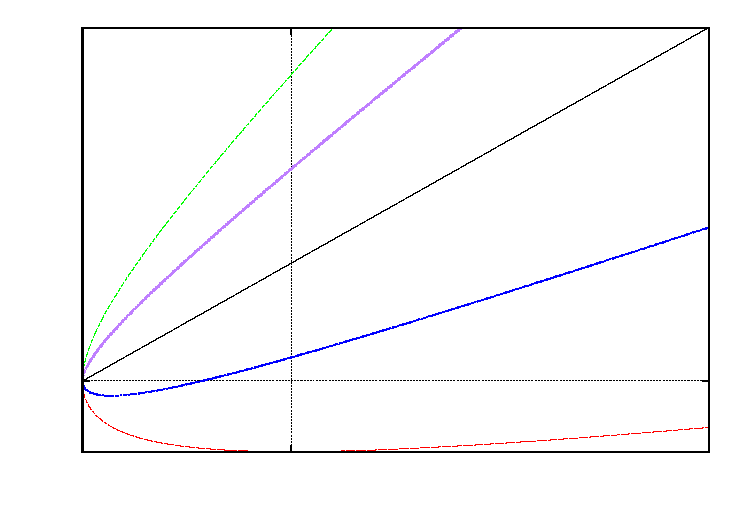
\includegraphics{chapters/neutron_interactions/incoming_outgoing_energies_cm_angle.pdf}}%
    \gplfronttext
  \end{picture}%
\endgroup

  \end{center}
  \caption{\textbf{Outgoing energy from forward reaction as a function of 
      incoming energy and center-of-mass scattering angle cosine}.
    \textit{For fixed incoming energy, there is a one-to-one correspondence
      between outgoing energy and center-of-mass scattering angle cosine. For
      fixed outgoing energy, there is only a one-to-one correspondence
      between incoming energy and center-of-mass scattering angle cosine if the
      outgoing energy is above $\frac{Q}{A(A+1)}$ or if the scattering angle
      cosine is above zero.}}
  \label{fig:in_out_energies_cm}
\end{figure}
\begin{figure}[t!]
  \begin{center}
    % GNUPLOT: LaTeX picture with Postscript
\begingroup
  \makeatletter
  \providecommand\color[2][]{%
    \GenericError{(gnuplot) \space\space\space\@spaces}{%
      Package color not loaded in conjunction with
      terminal option `colourtext'%
    }{See the gnuplot documentation for explanation.%
    }{Either use 'blacktext' in gnuplot or load the package
      color.sty in LaTeX.}%
    \renewcommand\color[2][]{}%
  }%
  \providecommand\includegraphics[2][]{%
    \GenericError{(gnuplot) \space\space\space\@spaces}{%
      Package graphicx or graphics not loaded%
    }{See the gnuplot documentation for explanation.%
    }{The gnuplot epslatex terminal needs graphicx.sty or graphics.sty.}%
    \renewcommand\includegraphics[2][]{}%
  }%
  \providecommand\rotatebox[2]{#2}%
  \@ifundefined{ifGPcolor}{%
    \newif\ifGPcolor
    \GPcolorfalse
  }{}%
  \@ifundefined{ifGPblacktext}{%
    \newif\ifGPblacktext
    \GPblacktexttrue
  }{}%
  % define a \g@addto@macro without @ in the name:
  \let\gplgaddtomacro\g@addto@macro
  % define empty templates for all commands taking text:
  \gdef\gplbacktext{}%
  \gdef\gplfronttext{}%
  \makeatother
  \ifGPblacktext
    % no textcolor at all
    \def\colorrgb#1{}%
    \def\colorgray#1{}%
  \else
    % gray or color?
    \ifGPcolor
      \def\colorrgb#1{\color[rgb]{#1}}%
      \def\colorgray#1{\color[gray]{#1}}%
      \expandafter\def\csname LTw\endcsname{\color{white}}%
      \expandafter\def\csname LTb\endcsname{\color{black}}%
      \expandafter\def\csname LTa\endcsname{\color{black}}%
      \expandafter\def\csname LT0\endcsname{\color[rgb]{1,0,0}}%
      \expandafter\def\csname LT1\endcsname{\color[rgb]{0,1,0}}%
      \expandafter\def\csname LT2\endcsname{\color[rgb]{0,0,1}}%
      \expandafter\def\csname LT3\endcsname{\color[rgb]{1,0,1}}%
      \expandafter\def\csname LT4\endcsname{\color[rgb]{0,1,1}}%
      \expandafter\def\csname LT5\endcsname{\color[rgb]{1,1,0}}%
      \expandafter\def\csname LT6\endcsname{\color[rgb]{0,0,0}}%
      \expandafter\def\csname LT7\endcsname{\color[rgb]{1,0.3,0}}%
      \expandafter\def\csname LT8\endcsname{\color[rgb]{0.5,0.5,0.5}}%
    \else
      % gray
      \def\colorrgb#1{\color{black}}%
      \def\colorgray#1{\color[gray]{#1}}%
      \expandafter\def\csname LTw\endcsname{\color{white}}%
      \expandafter\def\csname LTb\endcsname{\color{black}}%
      \expandafter\def\csname LTa\endcsname{\color{black}}%
      \expandafter\def\csname LT0\endcsname{\color{black}}%
      \expandafter\def\csname LT1\endcsname{\color{black}}%
      \expandafter\def\csname LT2\endcsname{\color{black}}%
      \expandafter\def\csname LT3\endcsname{\color{black}}%
      \expandafter\def\csname LT4\endcsname{\color{black}}%
      \expandafter\def\csname LT5\endcsname{\color{black}}%
      \expandafter\def\csname LT6\endcsname{\color{black}}%
      \expandafter\def\csname LT7\endcsname{\color{black}}%
      \expandafter\def\csname LT8\endcsname{\color{black}}%
    \fi
  \fi
  \setlength{\unitlength}{0.0500bp}%
  \begin{picture}(7200.00,5040.00)%
    \gplgaddtomacro\gplbacktext{%
      \csname LTb\endcsname%
      \put(792,484){\makebox(0,0){\strut{}$\frac{A+1}{A}Q$}}%
      \csname LTb\endcsname%
      \put(2796,484){\makebox(0,0){\strut{}$\frac{A}{A-1}Q$}}%
      \put(572,2739){\rotatebox{-270}{\makebox(0,0){\strut{}Outgoing Energy}}}%
      \put(3797,154){\makebox(0,0){\strut{}Incoming Energy}}%
      \put(6002,765){\makebox(0,0)[l]{\strut{}$^{\mu_{l} = -1}$}}%
      \put(5601,1355){\makebox(0,0)[l]{\strut{}$\mu_{l} = -\frac{1}{2}$}}%
      \put(5200,1925){\makebox(0,0)[l]{\strut{}$\mu_{l} = 0$}}%
      \put(3998,3228){\makebox(0,0)[l]{\strut{}$\mu_{l} = \frac{1}{2}$}}%
      \put(1593,4164){\makebox(0,0)[l]{\strut{}$\mu_{l} = 1$}}%
      \put(632,745){\makebox(0,0)[l]{\strut{}0}}%
    }%
    \gplgaddtomacro\gplfronttext{%
    }%
    \gplbacktext
    \put(0,0){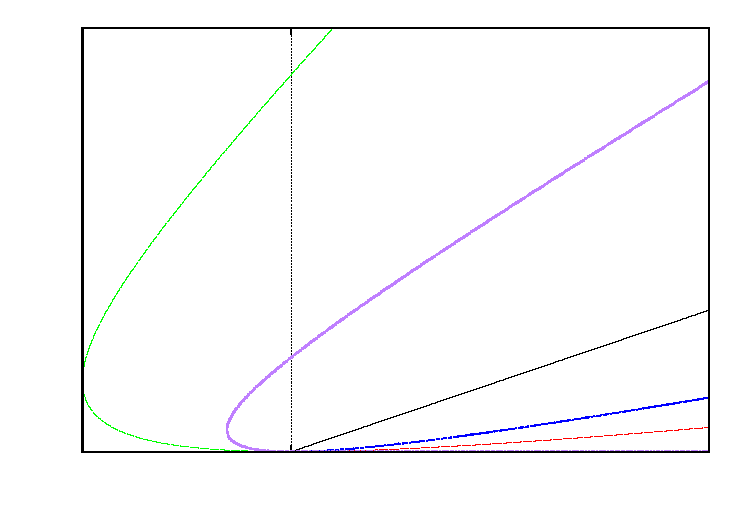
\includegraphics{chapters/neutron_interactions/incoming_outgoing_energies_lab_angle.pdf}}%
    \gplfronttext
  \end{picture}%
\endgroup

  \end{center}
  \caption{\textbf{Outgoing energy from forward reaction as a function of 
      incoming energy and lab scattering angle cosine}.
    \textit{For fixed incoming energy, there is only a one-to-one correspondence
      between outgoing energy and lab scattering angle cosine if the
      incoming energy is above $\frac{AQ}{A-1}$. For fixed outgoing energy,
      there is a one-to-one correspondence between incoming energy and lab
      scattering angle cosine.}}
  \label{fig:in_out_energies_cm}
\end{figure}
The incoming energy as a function of incoming energy and lab scattering angle
cosine is shown in the following equation. It must also be noted that the
primed and unprimed variables have been switched. The derivation of this 
equation is shown in appendix \ref{appendix_C}.
\begin{equation}
  E = E^{'}\left(\frac{A^2-1+2\mu_l^2 + A(A-1)\frac{Q}{E^{'}} - 
    2\mu_l\sqrt{A^2 - 1 + \mu_l^2 + A(A-1)\frac{Q}{E^{'}}}}{(A-1)^2}
  \right)
\end{equation}
By using $\mu_l = 1$ and $\mu_l = -1$ in the above equation, the lower and
upper energy bound of the adjoint elastic and inelastic level scattering
process can be determined, repsectively.
\begin{equation}
  \left(\frac{A\sqrt{1+\left(\frac{A-1}{A}\right)\frac{Q}{E^{'}}}-1}{A-1}
  \right)^2 E^{'} \leq E \leq
  \left(\frac{A\sqrt{1+\left(\frac{A-1}{A}\right)\frac{Q}{E^{'}}}+1}{A-1}
  \right)^2 E^{'}
\end{equation}

With the adjoint cross section for elastic and inelastic level scattering
completely defined, the adjoint energy transfer probability can now be 
determined using equation \ref{eq:adjoint_double_diff_transfer_prob}
\citep{hoogenboom_adjoint_1977}.
\begin{align}
  p^{\dagger}(E^{'} \to E) & = \frac{\sigma_{e/i}(E)p(E \to E^{'})}
  {\sigma_{e/i}^{\dagger}(E^{'})} \nonumber \\
    & = \frac{\sigma_{e/i}(E)}{\sigma_{e/i}^{\dagger}(E^{'})}
  \frac{(A+1)^2}{2AE\sqrt{1-\left(\frac{A+1}{A}\right)\frac{Q}{E}}}
  p(E, \mu_{cm}(E,E^{'})) 
\end{align}
Efficient methods for sampling from this function will be a major focus of this
work. However, it is likely that a tabular method will be used based on the
seemingly complex nature of this PDF.

Because of the one-to-one correspondence between the outgoing energy and
direction, once the outgoing energy has been selected the outgoing direction
is known. The following equation must be used to determine the outgoind
lab scattering angle cosine corresponding to the incoming and outgoing energy.
\begin{equation}
  \mu_l = - \left[\frac{\left(\frac{E}{E^{'}}\right)(A-1)^2 - 
      A^2\left(1+\left(\frac{A-1}{A}\right)\frac{Q}{E^{'}}\right) + 1}
    {2\sqrt{\frac{E}{E^{'}}}(A-1)}\right]
\end{equation}

\section{Other Non-fission Adjoint  Reactions}

\section{Adjoint Neutron Induced Fission}

\section{Adjoint Thermal Scattering}


